% !TEX root = ../bachlor-arbeit.tex
Before starting to implement anything we need to define which metasurface stacks the algorithm is allowed to produce. This was already partly motivated in the introduction: We want easy to manufacture metasurfaces which can produce a high variety of transmission spectra when stacked. Additionally, to keep things simple we want the transmission spectra to be the same for every point of entry along the base of the stack. Transmission spectra which also depend on the point of entry so $I = I(\lambda,x,y)$ can also be done \cite{Mueller2017} but functions $I = I(\lambda)$ are already useful and can represent for example a custom filter (the directions $x$ and $y$ are shown in figure \ref{fig:al:two_layers}).
With this in mind we are going to use a structure which is periodic in the
$x$ and $y$ direction and consists of one repeating meta-atom. These kind of surfaces can be manufactured via ... \note{ask jan how these are made}.
\\

$\quad$ As shown in section \ref{sec:SASA} paragraph \hyperref[sec:symmetries]{Symmetries} we cannot use meta-atoms of $C_4$ symmetry to produce different transmissions for the $x$ and $y$ polarization. The next simplest geometry is the rectangle. Another limitation given by the manufacturing process is the number of metasurface layers in a stack. Stacks with more than two layers become increasingly hard to manufacture that is why we are going to limit the algorithm to two-layer stacks even though theoretically arbitrary stacks could be used.
\\

\begin{figure}[H]
    \centering
    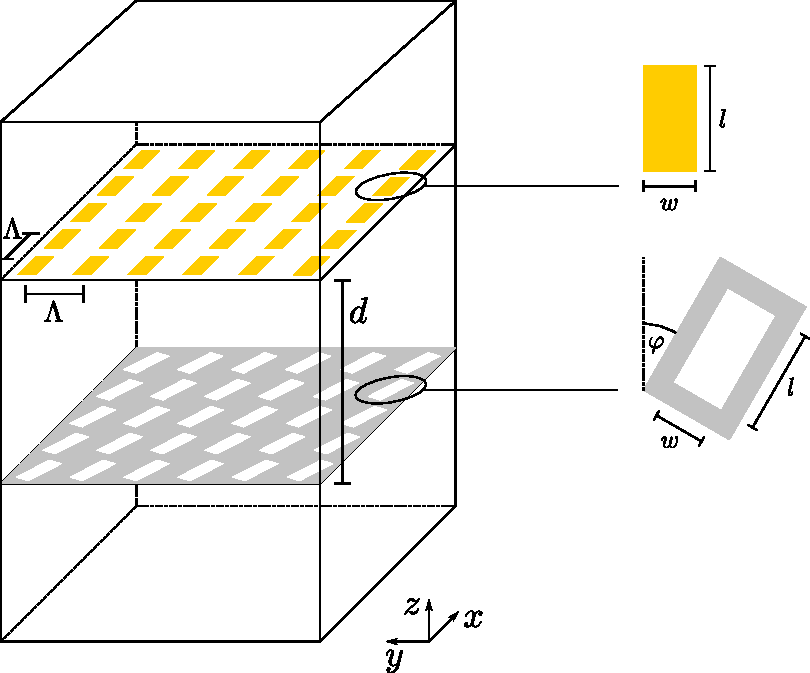
\includegraphics[width=.7\linewidth]{al_two_layers}
    \caption{A two layer stack to visualize all the design parameters
    $\mc D$ which can be set by the algorithm. These include stack parameters $\mc S$ and two sets of layer parameters $\mc L_1$ and $\mc L_2$.\\
    So $\mc D = (\mc S, \mc L_1, \mc L_2)$. The stack parameters consist of the distance between the metasurfaces $d$ and their rotation angle $\varphi$ so $\mc S = (d, \varphi)$. The layer parameters are the width $w$, length $l$ and thickness $t$ of the meta-atom, the period of meta-atoms $\Lambda$ the  material of the layer $m$ and the kind of geometry $g$. So $\mc L = (w,l,t,\Lambda,m,g)$. All of the parameters are continuous except the choice about the material and geometry.}
    \label{fig:al:two_layers}
\end{figure}


$\quad$ The last decision about the metasurfaces geometry is a little heuristic. A large variety of transmission spectra include some that are very absorbent everywhere except for specific wavelengths and some where almost all wavelengths are transmitted. A metal metasurface absorbs light when the electrons in the meta-atoms can oscillate in resonance. For rectangular meta-atoms this is the case for very specific wavelengths so metasurfaces made of these produce the former kind of spectrum. The opposite can be achieved when using rectangular holes. These metasurfaces have many different resonance frequencies and only the wavelengths that would have "fit" into the holes are not absorbed. That means the hole geometry can be used to produce the latter kind of spectrum and we have to include both geometries to reach the greatest variety.
As for the material we are going to limit the algorithm to Aluminium and Gold this is not physically motivated but we have to remember that every material we add multiplies the amount of metasurfaces that need to be simulated in preparation (see \textit{curse of dimensionality}) and more materials are only useful when the corresponding parameter space is sufficiently.
This ends the design considerations, a visualization of all parameters and the notation we are going to use referring to them can be found in figure \ref{fig:al:two_layers}.
